\section{Цель работы}
	Описать сценарии, которые реализует система.
	
\section{Диаграмма вариантов использования}


	\subsection{Диаграммы деятельности}
	
	
		\begin{figure}[ht] 
			\center
			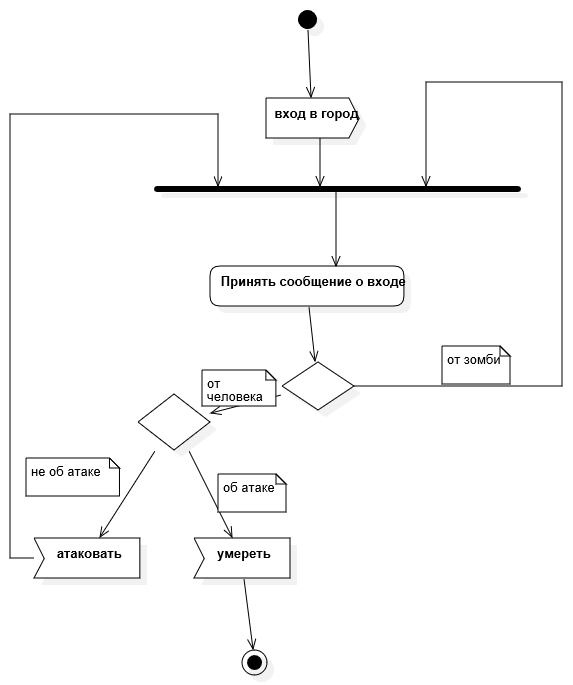
\includegraphics [width=0.6\textwidth] {zombie}
			\caption{Зомби} 
		\end{figure}
		
		\begin{figure}[ht] 
			\center
			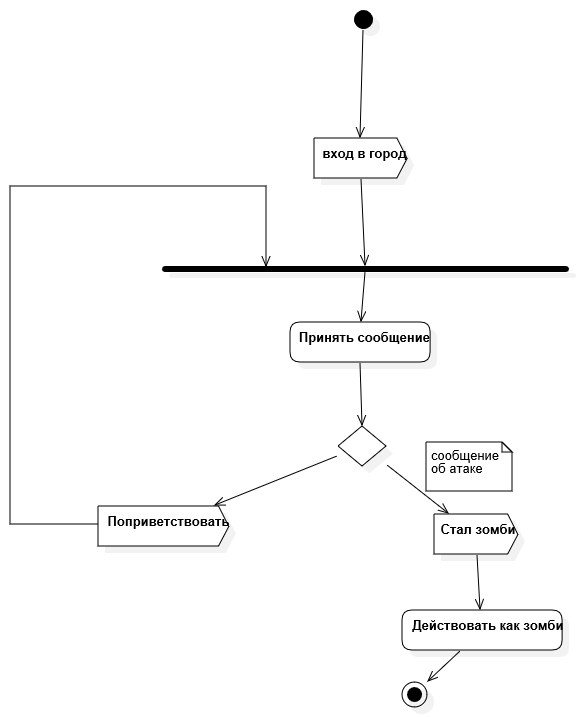
\includegraphics [width=0.4\textwidth] {not-knowing}
			\caption{Человек незнающий} 
		\end{figure}
	
		\begin{figure}[ht] 
			\center
			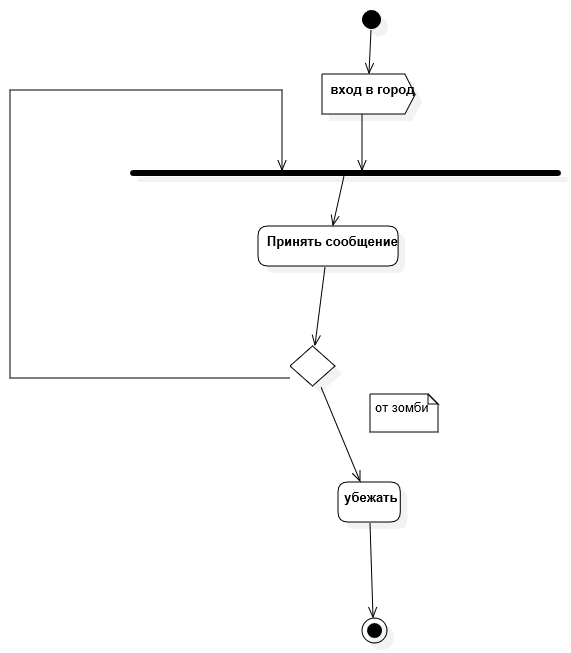
\includegraphics [width=0.4\textwidth] {knowing}
			\caption{Человек знающий} 
		\end{figure}
	
		\begin{figure}[ht] 
			\center
			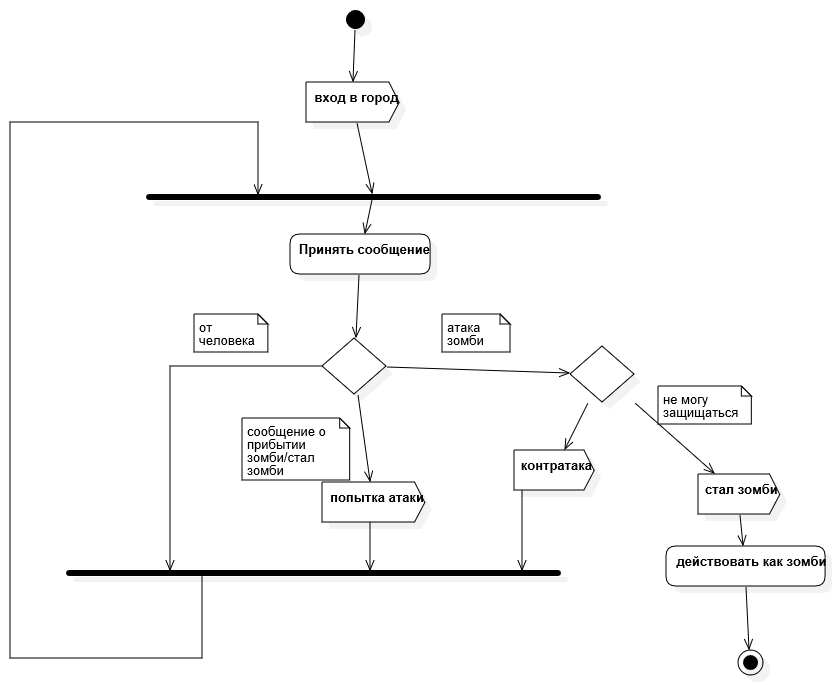
\includegraphics [width=0.8\textwidth] {defender}
			\caption{Защитник человечества} 
		\end{figure}

	
		\FloatBarrier
		\clearpage
	%\subsection{Диаграмма прецедентов}
		
	\subsection{Диаграммы последовательности}
			\begin{figure}[ht] 
				\center
				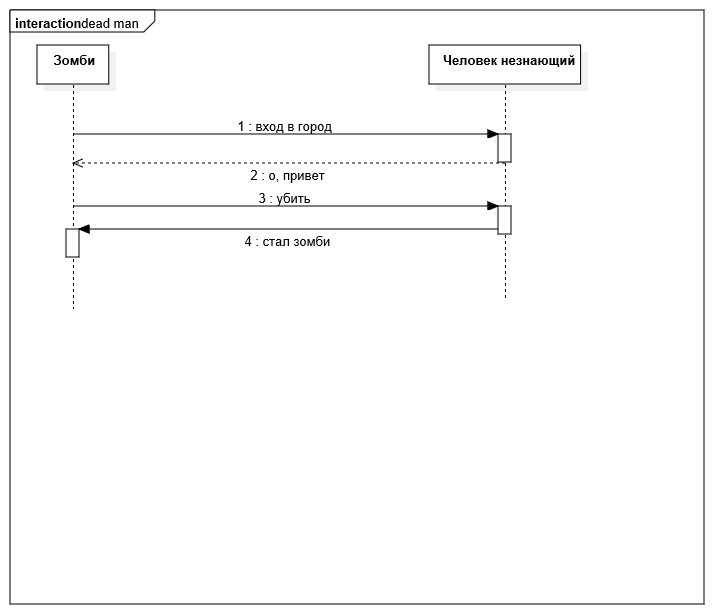
\includegraphics [width=0.5\textwidth] {inter_man}
				\caption{Зомби и незнающий}  
			\end{figure}
			
			\begin{figure}[ht] 
				\center
				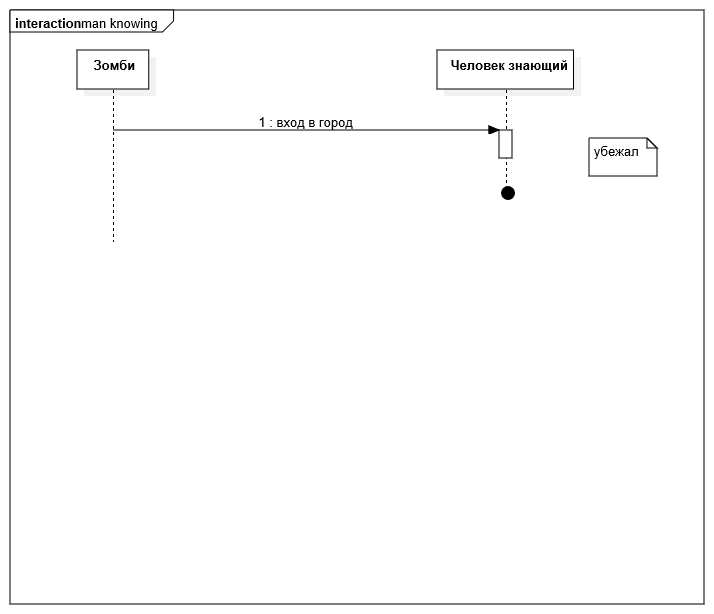
\includegraphics [width=0.5\textwidth] {inter_knowing}
				\caption{Зомби и знающий} 
			\end{figure}
			
			\begin{figure}[ht] 
				\center
				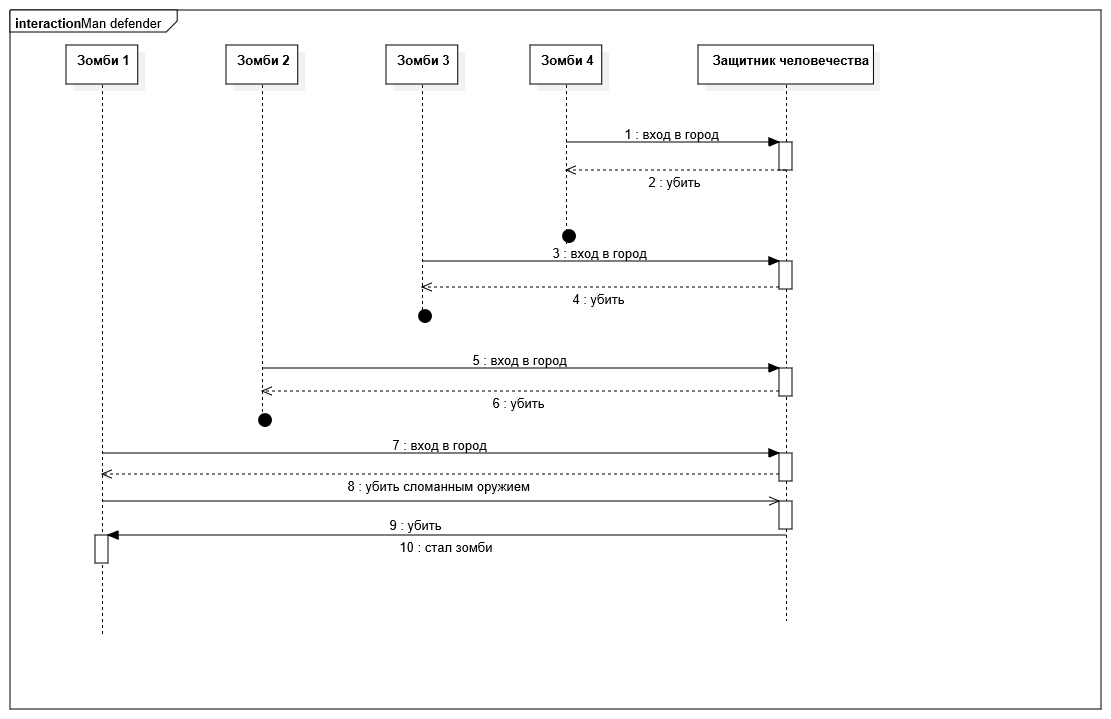
\includegraphics [width=0.6\textwidth] {inter_5}
				\caption{4 зомби и защитник человечества} 
			\end{figure}
			
			\begin{figure}[ht] 
				\center
				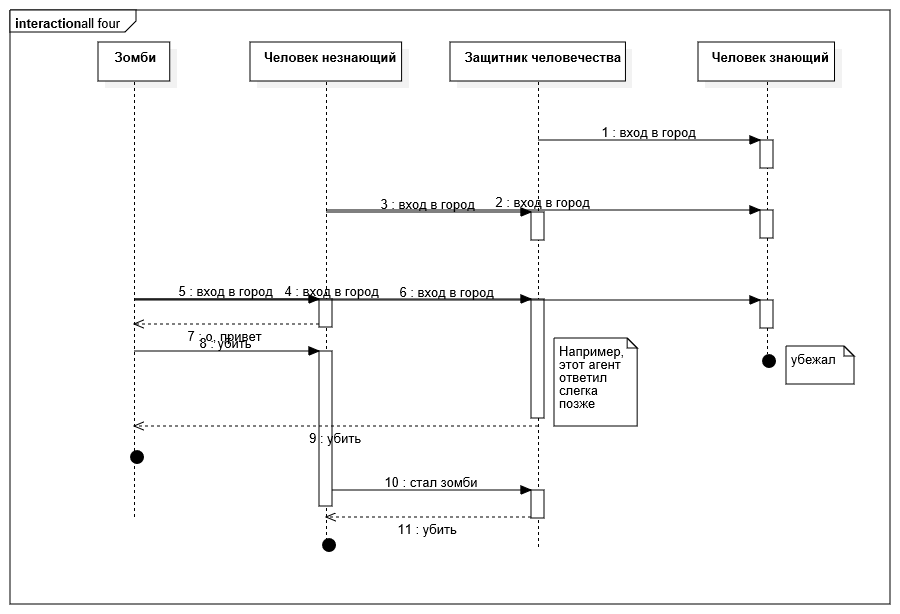
\includegraphics [width=0.6\textwidth] {inter_4}
				\caption{Сложное взаимодействие} 
			\end{figure}